\documentclass{standalone}
\usepackage{pgfplots}
\begin{document}
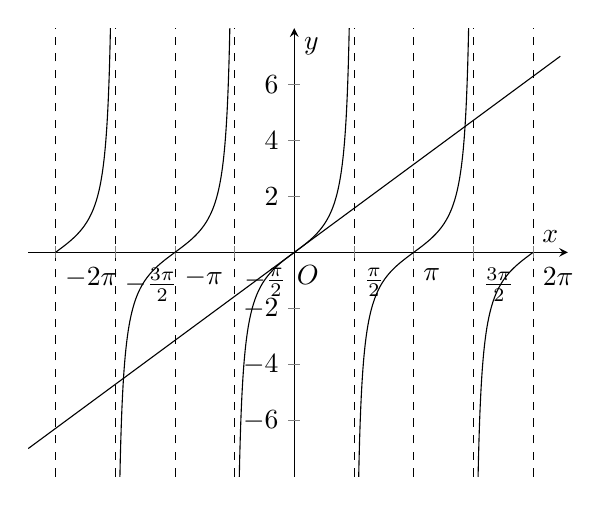
\begin{tikzpicture}
\begin{axis}
[
ymin=-8,ymax=8,
xmin=-7,xmax=7.2,
xtick=\empty,
ytick=\empty,
extra x ticks={-6.28319, -4.71239, -3.14159, -1.5708, 1.5708, 3.14159, 4.71239, 6.28319},
extra x tick labels={$-2\pi$, $-\frac{3\pi}{2}$, $-\pi$, $-\frac{\pi}{2}$, $\frac{\pi}{2}$, $\pi$, $\frac{3\pi}{2}$, $2\pi$},
extra y ticks={-6, -4, -2, 2, 4, 6},
extra y tick labels={$-6$, $-4$, $-2$, $2$, $4$, $6$},
every extra x tick/.style={
    xticklabel style={anchor=north west},
    grid=major,
    major grid style={very thin,dashed,black}
},
axis lines = center,
xlabel=$x$,ylabel=$y$,
samples=200,
]
\addplot [black, domain=-6.28319:-4.83239] {tan(deg(x))};
\addplot [black, domain=-4.59239:-1.6908] {tan(deg(x))};
\addplot [black, domain=-1.4508:1.4508] {tan(deg(x))};
\addplot [black, domain=1.6908:4.59239] {tan(deg(x))};
\addplot [black, domain=4.83239:6.28319] {tan(deg(x))};
\addplot [black, domain=-7:7] {x};
\node at (axis cs:0.355, -0.8) {$O$} ;
\end{axis}
\end{tikzpicture}
\end{document}
